\subsection{Decentralized Variance-Reduced SGF FW Experiments}
The experiments performed with Algorithm \ref{variance-reduced} were conducted considering $M=5$ workers. Each worker was fed with $S_1=800$ images (80 images per class) from the portion of the MNIST test set that LeNet5 was able to classify correctly. We imposed that the same image could not be assigned to different workers. This aspect was not clearly specified in the original algorithm proposed in \cite{A3}, section VI, in which the authors seem to suggest to use the same $S_1$ images for all the workers. However, the distributed data settings arise from the need of dividing huge datasets into different machines, for simplifying the computational complexity, and therefore we opted for an implementation choice that resulted more coherent with this idea.\\  The number $M$ of workers was halved compared to the one of the previous algorithm and also the other hyperparameters was chosen to be pretty low to reduce a bit the CPU-time consumption. In particular, we set the number of component functions to $n=5$ or $n=10$, the number of sampled components in RDSA to $S_2=3$, the number of queries to $T=20$ and the period parameter to $q=5$ or $q=7$ or $q=9$. With these settings, the algorithm approximatively took between one and four hours to terminate. In fact, the algorithm combines the hungry but accurate queries of KWSA, regulated by the parameter $q$, with the efficient but potentially inaccurate queries of RDSA. 
\begin{figure}[htbp]
	\centering
	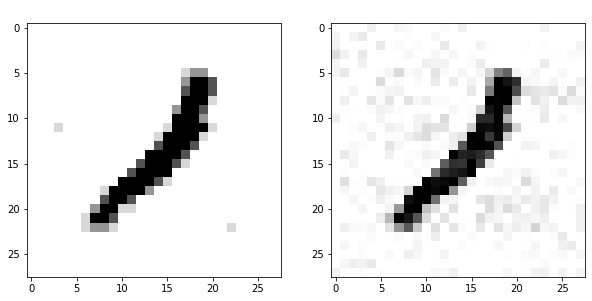
\includegraphics[width=7cm]{image_pertub_q5_n10_final.png}
	\caption{Image of 1 changed to 4 with the adversarial perturbation generated by the Decentralized Variance-Reduced Algorithm \ref{variance-reduced} with q=5 and n=10.}
	\label{fig:variance-reduced}
\end{figure}
In Figure \ref{fig:variance-reduced} we can see an example of the perturbations.
